A \textit{landing page} do projeto foi desenvolvida em \textit{HTML}, responsável pela estrutura do conteúdo, \textit{CSS}, utilizado para o estilo visual, e \textit{JavaScript}, empregado na implementação da interatividade e do dinamismo da navegação. O sistema de rastreamento ocular foi implementado em \textit{JavaScript}, utilizando a biblioteca \textit{WebGazer.js} \cite{papoutsaki2016webgazer}, que contém um modelo capaz de se autocalibrar ao observar a interação dos visitantes com a página, treinando um mapeamento entre as características do olhar e as posições na tela. O tratamento das coordenadas oculares recebidas do \textit{frontend} foi realizado em \textit{JavaScript}, com o uso do \textit{Node.js} e do \textit{Socket.IO}, possibilitando a comunicação em tempo real com o \textit{frontend}, uma vez que depende das coordenadas enviadas por ele. Essa parte do \textit{backend} é responsável por analisar métricas como acertos, erros por omissão, erros por comissão, tempo de reação e variabilidade temporal das respostas, dados que serão utilizados para compor o feedback individual de cada usuário. Por fim, o jogo \textit{web} foi desenvolvido em \textit{TypeScript}, utilizando o \textit{framework} \textit{Next.js}, o que proporcionou um código mais robusto, organizado e uma experiência de uso moderna e fluida.

A metodologia fundamenta-se na aplicação adaptada do TDC. A principal diferença do presente trabalho está na integração do teste com o rastreamento ocular em tempo real, permitindo a coleta de dados visuais complementares durante a execução das tarefas.

O experimento é estruturado como um jogo digital de temática espacial, composto por
três fases com níveis crescentes de dificuldade. A mecânica de jogo foi desenhada para simular os
princípios do TDC, promovendo a exposição contínua a estímulos visuais por períodos prolongados e exigindo respostas rápidas e consistentes por parte do participante. Ao longo de cada fase, o sistema registra métricas relacionadas à atenção, como erros de omissão (quando o participante não responde a um estímulo-alvo), erros de comissão (quando não mantém foco por tempo suficiente no alvo), tempo de reação e variabilidade temporal das respostas.

Durante toda a experiência, o rastreamento ocular é realizado em segundo plano, utilizando
bibliotecas como o \textit{WebGazer} para capturar os pontos de fixação visual do usuário por meio da \textit{webcam}. Esses dados permitem identificar padrões de atenção ou desatenção de acordo com nossa base de dados em cada etapa da atividade. Todas as fases contam com música de fundo, cuja intensidade e ritmo são ajustados conforme o nível de dificuldade, de forma a potencializar a sobrecarga sensorial e dificultar a concentração.

A pesquisa de dados estatísticos foi conduzida por meio de um formulário composto por cinco questões, o qual foi respondido por cinco profissionais da área da Psicologia. No que se refere aos estímulos visuais empregados para a detecção de indícios de desatenção em crianças, os participantes destacaram que fatores como foco, tempo, som, cores e movimento constituem parâmetros relevantes para essa finalidade. Em virtude dessas considerações, tais elementos foram incorporados em todas as etapas do jogo desenvolvido. Ademais, todos os profissionais consultados reconheceram o rastreamento ocular como uma ferramenta útil, indicando que sua aplicação no contexto da abordagem proposta apresenta potencial para contribuir de forma eficaz na identificação de comportamentos relacionados à desatenção. Por fim, foram registradas sugestões de aprimoramento metodológico, como redirecionar o foco do estudo para uma aplicação de caráter clínico, inserir uma fase com estímulos \textit{distractors}, seguida de questionamentos específicos sobre o conteúdo \textit{distractor}, bem como assegurar que os estímulos sejam facilmente reconhecíveis pelas crianças participantes.

\begin{figure}[H]
    \centering
    \caption{Primeira fase}%
    \label{fig:primeira-fase}
    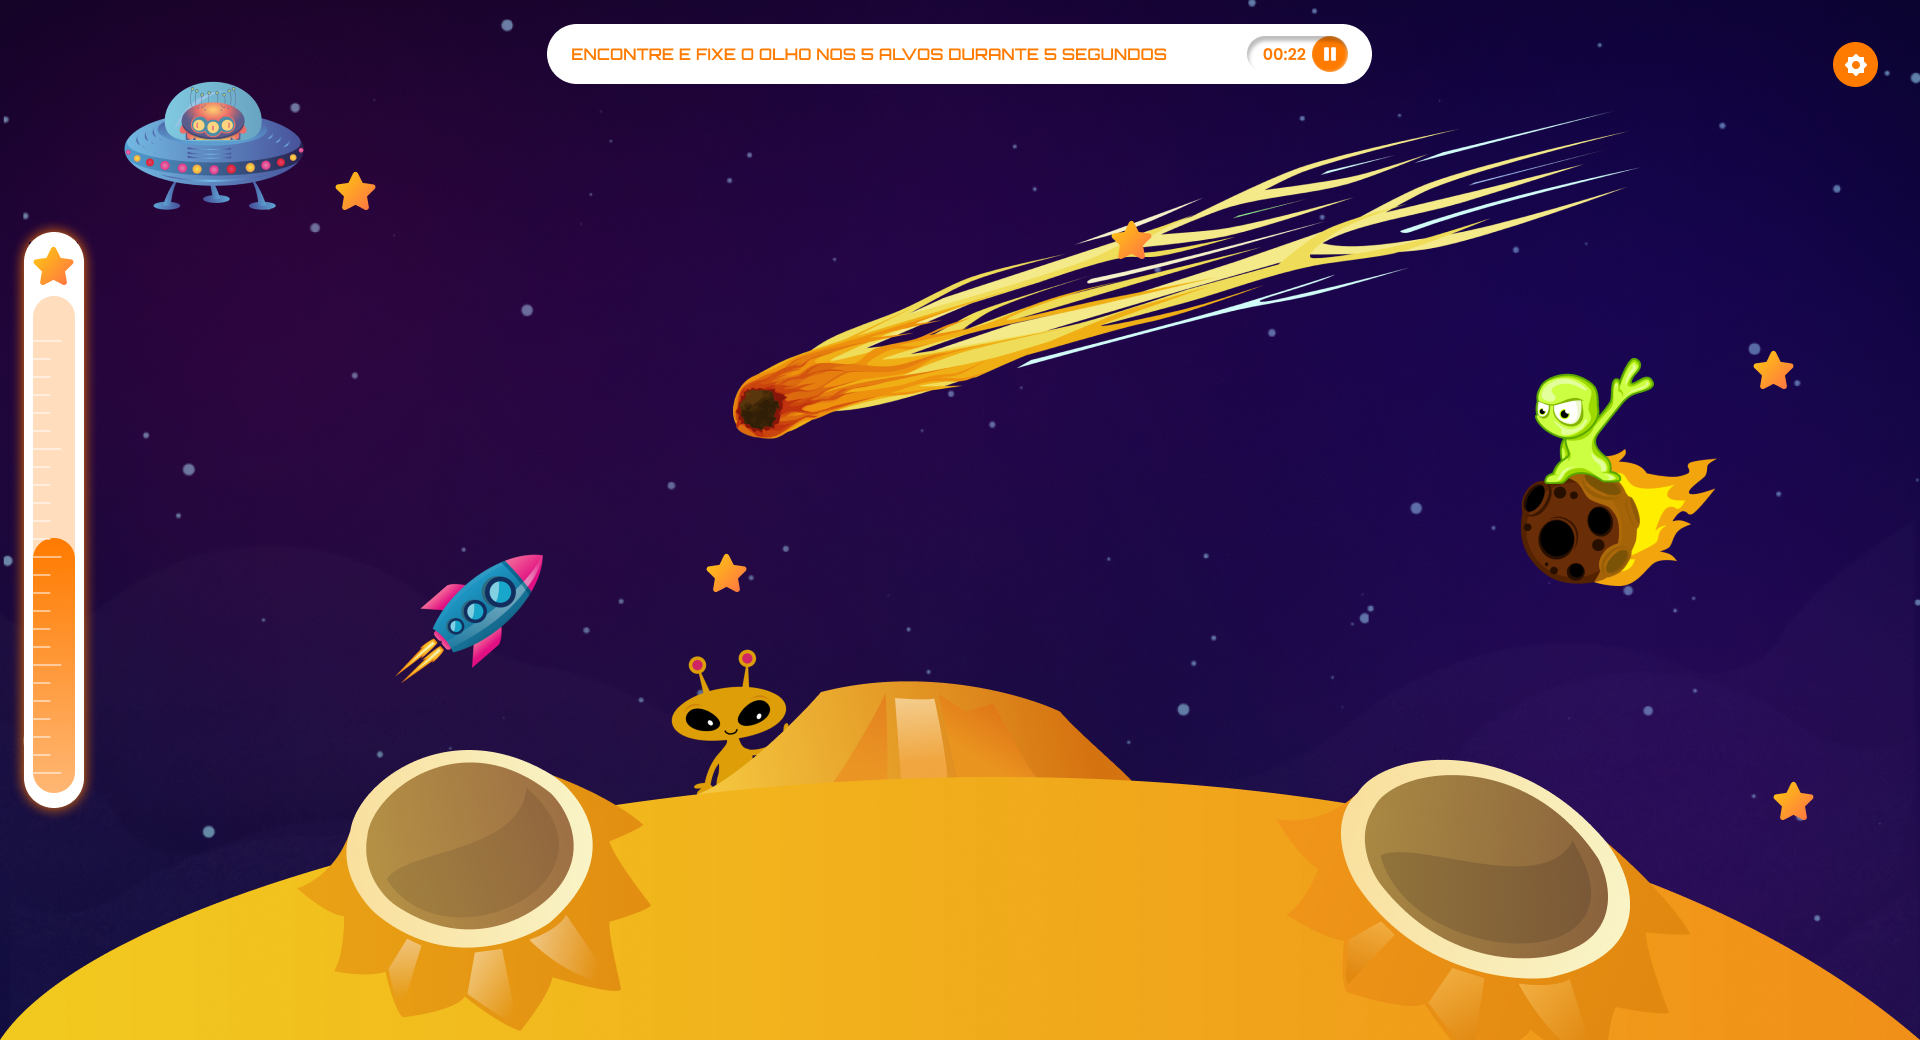
\includegraphics[width=\textwidth]{primeira-fase.png}%
    \SourceOrNote{Autoria Própria (2024)}
\end{figure}

Na primeira fase, o participante deve fixar o olhar por cinco segundos em cinco alvos estáticos,
representados por estrelas, enquanto elementos animados surgem ao redor. Após os 5 segundos,
cada estrela desaparece da tela. A música de fundo nesta etapa apresenta um ritmo moderado. O
objetivo é avaliar a capacidade de manter a atenção em um ponto fixo durante um tempo determinado, ignorando estímulos visuais e auditivos periféricos.

\begin{figure}[H]
    \centering
    \caption{Segunda fase}%
    \label{fig:segunda-fase}
    \SourceOrNote{Autoria Própria (2024)}
\end{figure}

Na segunda fase, são apresentadas cinco estrelas estáticas, que brilham individualmente em sequência, enquanto três planetas transitam pela tela, atuando como estímulos secundários que o participante deve acompanhar visualmente durante o movimento. Ao término da fase, o usuário responde a um formulário composto por perguntas relacionadas aos planetas observados, utilizando botões \textit{IoT}, cada um correspondente a um planeta específico. Essa etapa tem como objetivo mensurar a rastreabilidade ocular, exigindo que o participante direcione o olhar aos planetas em movimento contínuo pela tela. A trilha sonora torna-se mais intensa e acelerada nesta fase, com o propósito de aumentar o nível de exigência atencional e avaliar a capacidade de concentração diante de múltiplos estímulos visuais e auditivos.

\begin{figure}[H]
    \centering
    \caption{Terceira fase}%
    \label{fig:terceira-fase}
    \SourceOrNote{Autoria Própria (2024)}
\end{figure}

Na terceira fase, a demanda cognitiva é intensificada pela necessidade de alternância rápida do foco visual entre diferentes regiões da tela, caracterizadas por menor previsibilidade espacial. Nessa etapa, uma estrela surge de forma estática, exigindo resposta ocular imediata do participante. Simultaneamente, um segundo estímulo estático é apresentado, alternando entre os estados ligado e desligado em intervalos regulares. Quando esse estímulo é ativado (ascende), o participante deve manter o olhar fixo sobre ele até que se apague, o que permite avaliar a atenção sustentada e o controle do direcionamento ocular. A trilha sonora atinge seu nível máximo de intensidade e agitação, contribuindo para aumentar a complexidade da tarefa. O desempenho do participante nesta fase é utilizado como indicador da agilidade atencional e da capacidade de redirecionamento e manutenção do foco visual diante de estímulos dinâmicos.

Ao término das três fases, o sistema apresenta ao participante um resumo dos resultados com base em métricas como número de acertos, erros por omissão, erros por comissão e tempo médio de reação. Para isso, são utilizados os três registros mais recentes de rastreamento ocular, que correspondem às três fases concluídas pelo jogador. Com base nesses dados, o sistema gera um feedback textual interpretativo, apresentando mensagens como: “Sua atenção está conforme o esperado”, “Sua atenção está acima do esperado” ou “Sua atenção está abaixo do esperado.”, de acordo com o desempenho observado.

A plataforma é desenvolvida com tecnologias \textit{web}, permitindo acesso remoto e execução
direta em \textit{browsers} modernos. O teste é realizado de forma autônoma pelo usuário, em ambiente silencioso e seguindo instruções fornecidas pela própria plataforma.

Para melhor compreensão da sequência lógica do teste, a Figura \ref{fig:fluxograma-jogo} ilustra o fluxo de execução da plataforma desde o acesso inicial até a geração do feedback final. O \textit{flowchart} apresenta as etapas do experimento, desde o momento em que o usuário acessa o sistema e recebe instruções sobre o funcionamento do jogo, até a execução da primeira fase, baseada no \textit{Continuous Performance Test}. Nessa fase, são introduzidos estímulos visuais \textit{distractors}, e a plataforma registra o foco ocular do usuário utilizando visão computacional. A partir disso, os dados coletados — como desvios de atenção, acertos, erros e omissões — são analisados e comparados com uma base de dados para que o sistema gere um feedback interpretativo personalizado ao participante.

\begin{figure}[H]
    \centering
    \caption{Fluxograma do jogo}%
    \label{fig:fluxograma-jogo}
    \SourceOrNote{Autoria Própria (2024)}
\end{figure}

Optou-se pela utilização do banco de dados não relacional \textit{MongoDB}, o qual armazena informações em documentos no formato \textit{JSON}, possibilitando a criação de estruturas dinâmicas e aninhadas, adequadas ao armazenamento dos dados provenientes dos testes de rastreamento ocular. Sua flexibilidade e escalabilidade o tornam mais apropriado que bancos relacionais para o tratamento de grandes volumes de dados sensoriais. O gerenciamento do banco foi realizado por meio do \textit{MongoDB Compass}, ferramenta que facilita a execução de consultas, validação de esquemas e análise de desempenho.
